\documentclass{summarysheet}

\begin{document}


\maketitle{4}{Gauss's Law}

\begin{multicols}{2}

\begin{topicbox}{Symmetry}

\noindent A charge distribution is symmetric if it is unchanged following a translation, rotation, or reflection.

\begin{teqbox}
\textbf{The symmetry of the electric field must match the symmetry of the charge distribution.}
\end{teqbox}

\noindent There are three main symmetries we’ll encounter:
\begin{center}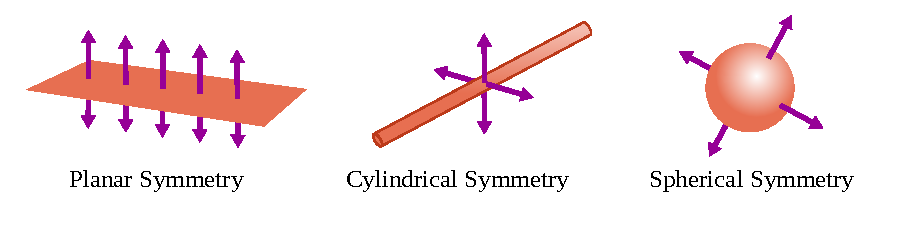
\includegraphics[scale=0.6]{fig_symmetries.pdf}\end{center}

\end{topicbox}


\begin{topicbox}{Electric Flux}
\begin{multicols}{2}
\noindent The electric flux $\Phi_\text{E}$ is, loosely speaking, how much of the electric field $\vec{E}$ ``flows through'' an area $A$. Mathematically,
\[
\Phi_\text{E} = \int_\text{surface} \vec{E} \cdot d\vec{A}.
\]
\begin{center}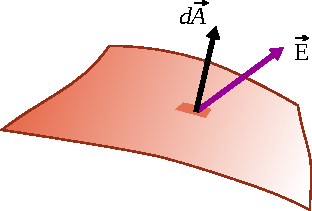
\includegraphics[scale=0.6]{fig_flux.pdf}\end{center}

\end{multicols}

\noindent If the electric field is everywhere tangent to the area, $\Phi_\text{E} = 0$. If the electric field is everywhere perpendicular to the area,

\[
\Phi_\text{E} = \int_\text{surface} E \, dA.
\]

\noindent If the electric field is perpendicular and is constant in magnitude along the surface,
\[
\Phi_\text{E} = EA.
\]

\end{topicbox}

\end{multicols}

\begin{topicbox}{Gauss's Law}

\noindent The net electric flux through a closed surface enclosing charge $Q_\text{in}$ is
\begin{teqbox}
\[
\Phi_\text{E} = \oint \vec{E} \cdot d\vec{A} = \frac{Q_\text{in}}{\epsilon_0}.
\]
\end{teqbox}

\end{topicbox}


\begin{multicols}{2}

\begin{topicbox}{Gaussian Surfaces}

\noindent When working with Gauss’s Law, we draw an imaginary closed surface around charge called a \emph{Gaussian surface}. The electric flux is calculated for this surface.

\begin{center}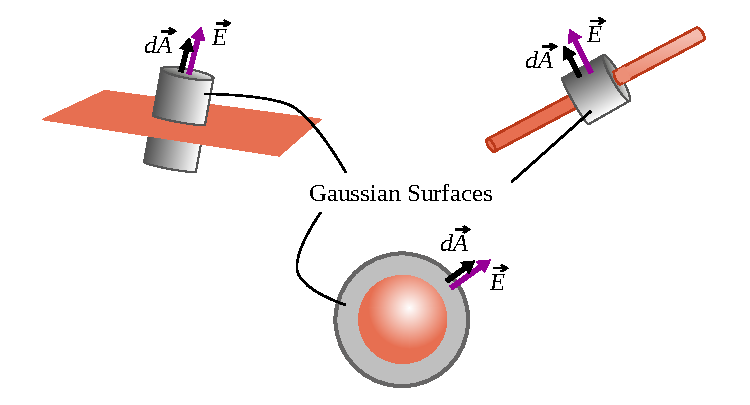
\includegraphics[scale=0.6]{fig_surface.pdf}\end{center}

\end{topicbox}

\begin{topicbox}{Problem-Solving Strategy}

\begin{itemize}
\item Determine the symmetry of the problem; if it’s planar, cylindrical, or spherical, use Gauss’s law.
\item Draw a Gaussian surface of the same symmetry (using a cylinder or sphere). Make it as large as you need to.
\item Determine the flux through the Gaussian surface; remember to use the size of the Gaussian surface, not the object itself.
\item Determine the enclosed charge $Q_\text{in}$; depending on the situation, you might have to use the charge density and the enclosed length, area, or volume:
\[
Q_\text{in} = \lambda L, \quad Q_\text{in} = \eta A, \quad \text{or} \quad  Q_\text{in} = \rho V.
\]
\item Use Gauss’s law to equate the flux with the enclosed charge (divided by $\epsilon_0$).  Solve for what you’re looking for.
\end{itemize}

\end{topicbox}

\end{multicols}

\begin{topicbox}{Conductors}
\begin{multicols}{2}

Gauss’s law allows us to make certain conclusions about \emph{electric fields} and \emph{conductors}.  
\begin{itemize}
\item The Electric field is zero within a conductor.
\item Any excess charge exists on the exterior surface.
\item The electric field is zero within any hole in the conductor (unless there is charge in the hole).
\item The electric field is perpendicular to the surface of a conductor.
\end{itemize}
\begin{center}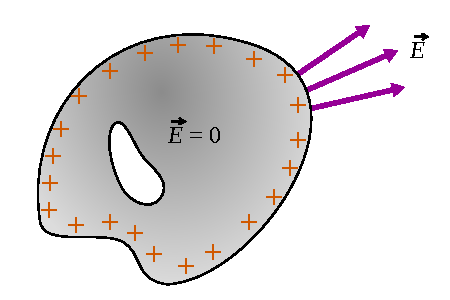
\includegraphics[scale=0.7]{fig_conductor.pdf}\end{center}
\end{multicols}
\end{topicbox}


\makebanner{Electricity and Magnetism}

\end{document}



